% 2013 湖南卷文科第 18 题：直角边长为 4 的格点三角形地块。
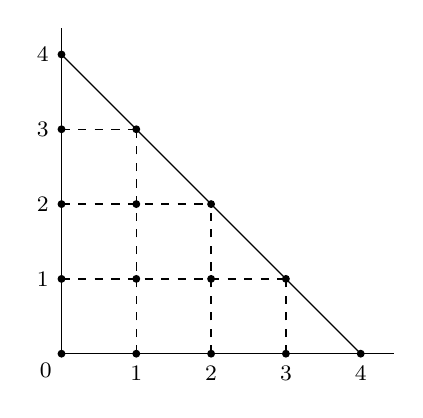
\begin{tikzpicture}[font=\footnotesize, line width=0.45pt, scale=0.95]
  % 坐标轴
  \draw (0,0) -- (4.45,0);
  \draw (0,0) -- (0,4.35);
  % 三角形边界（斜边）
  \draw (0,4) -- (4,0);
  % 三角形内的格线
  \begin{scope}
    \clip (0,0) -- (4,0) -- (0,4) -- cycle;
    \draw[dashed] (0,1) -- (4,1) (0,2) -- (4,2) (0,3) -- (4,3)
                  (1,0) -- (1,4) (2,0) -- (2,4) (3,0) -- (3,4);
  \end{scope}
  % 格点（共 15 个）
  \foreach \x in {0,...,4} {
    \foreach \y in {0,...,4} {
      \pgfmathparse{int(\x+\y<=4)}\ifnum\pgfmathresult=1
        \fill (\x,\y) circle (1.5pt);
      \fi
    }
  }
  % 刻度数字
  \foreach \x in {1,...,4} {
    \node[below] at (\x,-0.04) {$\x$};
  }
  \foreach \y in {1,...,4} {
    \node[left] at (-0.04,\y) {$\y$};
  }
  \node[below left] at (0,0) {$0$};
\end{tikzpicture}
